\section{Offline IRL/DDC experiments}\label{sec:Experiments}


We now present results from simulation experiments, in which we compare the performance of our approach against a series of benchmark algorithms. 
 
In the main text, we use the high-dimensional version of the canonical bus engine replacement problem (\cite{rust1994structural}) as the setting for our experiments. This setting has been extensively used as the standard benchmark for the reward learning problem in the DDC literature in economics \citep{hotz1993conditional, aguirregabiria2002swapping,  kasahara2009nonparametric,  arcidiacono2011conditional,  arcidiacono2011practical, su2012constrained, norets2009inference, chiong2016duality, reich2018divide, chernozhukov2022locally, geng2023data, barzegary2022recursive, yang2024estimation}. 

In addition, in Appendix \ref{sec:ExtendedExp}, for completeness, we also provide OpenAI gym benchmark environment experiments with a discrete action space (Lunar Lander, Acrobot, and Cartpole) \cite{brockman2016openai} as in \citet{garg2021iq} for the related, but easier problem of imitation learning. 

\subsection{Experimental Setup}
The bus engine replacement problem \cite{rust1987optimal} is a simple regenerative optimal stopping problem. In this setting, the manager of a bus company operates many identical buses. As a bus accumulates mileage, its per-period maintenance cost increases. The manager can replace the engine in any period (which then becomes as good, and this replacement decision re-sets the mileage to one). However, the replacement decision comes with a high fixed cost. Each period, the manager makes a dynamic trade-off between either replacing the engine or continuing with maintenance. We observe the manager's decisions for a fixed set of buses, i.e., a series of states, decisions, and state transitions. Our goal is to learn the manager's reward function from these observed trajectories under the assumption that he made these decisions optimally. 

\noindent \textbf{Dataset.} 
There are $N$ independent and identical buses (trajectories) indexed by $j$, each of which has $100$ periods over which we observe them, i.e., $h\in\{1\ldots 100\}$. Each bus's trajectory starts with an initial mileage of 1. The only reward-relevant state variable at period $h$ is the mileage of bus $x_{jh} \in \{1, 2, \ldots 20\}$. 

\noindent \textbf{Decisions and rewards.}\;\; There are two possible decisions at each period, replacement or continuation, denoted by $d_{jh} = \{0,1\}$. $d_{jh}=1$ denotes replacement, and there is a fixed cost $\theta_1$ of replacement. Replacement resets the mileage to 1, i.e., the engine is as good as new. $d_{jh}=0$ denotes maintenance, and the cost of maintaining the engine depends on the mileage as follows: $\theta_0 x_{jh}$. Intuitively, the manager can pay a high fixed cost $\theta_1$ for replacing an engine in this period but doing so reduces future maintenance costs since the mileage is reset to 1. In all our experiments, we set $\theta_0 = 1$ (maintenance cost) and $\theta_1 = 5$ (replacement cost). Additionally, we set the discount factor to $\beta = 0.95$.

\noindent \textbf{State transitions at each period.}\;\; If the manager chooses maintenance, the mileage advances by 1, 2, 3, or 4 with a $1/4$ probability each. If the manager chooses to replace the engine, then the mileage is reset to 1. That is, $\mathbb{P}(\{x_{j(h+1)}=x_{jh}+k\}\mid d_{jh}=0 ) = 1/4$, $k\in \{1,2,3,4\}$ and $\mathbb{P}\{x_{j(h+1)}=1\mid d_{jh}=1\}=1$. When the bus reaches the maximum mileage of 20, we assume that mileage remains at 20 even if the manager continues to choose maintenance.

%The cost for choosing action $d_{jh}$ depends only on how much mileage bus $j$ accumulated from its last replacement of the engine $x_{jt}\in \mathcal{S}=\{1, 2, \ldots 20\}$: when the manager decides to keep the engine with mileage $x_{jt}$, maintenance cost occurs with the amount $\theta_1 x_{jt}$; footnote{In DDC notation, this is equivalent to maintenance cost of $\theta_1 x_{j t}+\epsilon_{j t 0}$ and replacement cost of $\theta_2+\epsilon_{jt1}$, where $\epsilon_{jt0}, \epsilon_{jt1}$ are both independently and identically drawn from $G(0, 1)$ for $h\in [H]$ and $j\in [N]$, where $G$ is the Type 1 Extreme Value (T1EV) distribution. }. 

%This reward information is not revealed to the researcher. 

\noindent \textbf{High-dimensional setup.}\;\; In some simulations, we consider a high-dimensional version of the problem, where we now modify the basic set-up described above to include a set of $K$ high-dimensional state variables, similar to \citet{geng2023data}. Assume that we have access to an additional set of $K$ state variables $\{s^1_{jh}, s^2_{jh}, s^3_{jh} \ldots s^K_{jh}\}$, where each $s^k_{jh}$ is an i.i.d random draw from $\{-10, -9, \ldots, 9, 10\}$. We vary $K$ from 2 to 100 in our empirical experiments to test the sensitivity of our approach to the dimensionality of the problem.   
Further, we assume that these high-dimensional state variables $s_{jh}^k$s do not affect the reward function or the mileage transition probabilities. However, the researcher does not know this. So, they are included in the state space, and ideally, our algorithm should be able to infer that these state variables do not affect rewards and/or value function and recover the true reward function.

\noindent \textbf{Traing/testing split.}  Throughout, we keep 80\% of the trajectories in any experiment for training/learning the reward function, and the remaining 20\% is used for evaluation/testing. 

\noindent \textbf{Functional form.} For all non-parametric estimation methods (including ours), we used a multi-layer perception (MLP) with two hidden layers and 10 perceptrons for each hidden layer for the estimation of $Q$-function. For parametric-oracle methods, we use the reward functions' true parametric form (as described earlier).

\subsection{Benchmark Algorithms}
We compare our algorithm against a series of standard, or state-of-art benchmark algorithms in the DDC and IRL settings.
\\
\textbf{Rust (Oracle)}
\; Rust is an oracle-like fixed point iteration baseline that uses the nested fixed point algorithm \citep{rust1987optimal}. It assumes the knowledge of: (1) linear parametrization of rewards by $\theta_1$ and $\theta_2$ as described above, and (2) the exact transition probabilities. 
\\
\textbf{ML-IRL (Oracle)}\; ML-IRL from \citet{zeng2023understanding} is the state-of-art offline IRL algorithm that minimizes negative log-likelihood of choice (i.e., the first term in Equation \eqref{eq:mainopt}). This method requires a separate estimation of transition probabilities, which is challenging in high-dimensional settings. So, we make the same Oracle assumptions as we did for Rust (Oracle), i.e., assume that transition probabilities are known. Additionally, to further improve this method, we leverage the finite dependence property of the problem \cite{arcidiacono2011conditional}, which helps avoid roll-outs.  
\\
\textbf{SAmQ}\; SAmQ \cite{geng2023data} fits approximated soft-max Value Iteration (VI) to the observed data. We use the SAmQ implementation provided by the authors\footnote{\href{https://github.com/gengsinong/SAmQ}{https://github.com/gengsinong/SAmQ}}; their code did not scale due to a memory overflow issue for the trajectories larger than 2500, i.e., 250,000 samples. %Here s-s are going in 
\\
\textbf{IQ-learn}\; IQ-learn is a popular gradient-based method, maximizing occupancy matching objective (which does not guarantee that the Bellman equation is satisfied -- See Section \ref{sec:occupancy}).
\\
\textbf{BC}\; Behavioral Cloning (BC) simply minimizes the expected negative log-likelihood. This simple algorithm outperforms \cite{zeng2023understanding, li2022rethinkingvaluedice} many recent algorithms such as ValueDICE \cite{kostrikov2019imitation}. For details, see discussions in Section \ref{sec:ERM-IRL}.

\subsection{Experiment results}%\todo{Should write more}
\subsubsection{Performance results for the standard bus engine setting}
Table \ref{fig:mse_r_estimation} provides a table of simulation experiment results without dummy variables, i.e., with only mileage ($x_{jh}$) as the relevant state variable. The performance of algorithms was compared in terms of \textit{mean absolute percentage error (MAPE)} of $r$ estimation, which is defined as $\frac{1}{N} \sum_{i=1}^N \left|\frac{\hat{r}_i-r_i}{r_i}\right| \times 100$, where $N$ is the total number of samples from expert policy $\pi^*$ and $\hat{r}_i$ is each algorithm's estimator for the true reward $r_i$.\footnote{In the simulation we consider, we don't have a state-action pair with true reward near 0.}\footnote{As we assume that the data was collected from agents following (entropy regularized) optimal policy $\pi^*$ (Assumption \ref{ass:IRLoptimaldecision}), the distribution of states and actions in the data is the best data distribution choice.} 


\begin{table*}[h]
    \centering
    \scalebox{0.8}{
    \begin{tabular}{l
            >{\centering\arraybackslash}p{2.5cm}
            >{\centering\arraybackslash}p{2.5cm}
            >{\centering\arraybackslash}p{2.5cm}
            >{\centering\arraybackslash}p{2.5cm}
            >{\centering\arraybackslash}p{2.5cm}
            >{\centering\arraybackslash}p{2.5cm}}
\toprule
\multirow{2}{*}{\parbox{1.7cm}{No. of Trajectories\\(H=100)}} 
& \multicolumn{2}{c}{Oracle Baselines} & \multicolumn{4}{c}{\makecell{Nonparametric, No Knowledge of Transition Probabilities
}} \\
\cmidrule(lr){2-3} \cmidrule(lr){4-7}
& Rust & ML-IRL & \textbf{\ul{GLADIUS}} & SAmQ & IQ-learn & BC \\
\cmidrule(lr){2-7}
& MAPE (SE) & MAPE (SE) & MAPE (SE) & MAPE (SE) & MAPE (SE) & MAPE (SE) \\
\midrule
50   & 3.62 (1.70) & 3.62 (1.74) & \textbf{3.44} (1.28) & 4.92 (1.20)  & 114.13 (26.60) & 80.55 (12.82)  \\
250   & 1.37 (0.77) & 1.10 (0.78) & \textbf{0.84} (0.51) & 3.65 (1.00)  & 112.86 (27.31) & 72.04 (13.21) \\
500   & 0.90 (0.56) & 0.84 (0.59) & \textbf{0.55} (0.20) & 3.13 (0.86)  & 113.27 (25.54) & 71.92 (12.44) \\
1000  & 0.71 (0.49) & 0.64 (0.48) & \textbf{0.52} (0.22) & 1.55 (0.46)  & 112.98 (24.12) & 72.17 (12.11) \\
2500  & 0.68 (0.22) & 0.62 (0.35) & \textbf{0.13} (0.06) & N/A          & 111.77 (23.99) & 62.61 (10.75) \\
5000  & 0.40 (0.06) & 0.43 (0.26) & \textbf{0.12} (0.06) & N/A          & 119.18 (22.55) & 46.45 (8.22) \\
\bottomrule
\multicolumn{7}{l}{\footnotesize 
Based on 20 repetitions. Oracle baselines (Rust, MLIRL) were based on bootstrap repetition of 100.}
\end{tabular}
    }
\caption{Mean Absolute Percentage Error (MAPE) (\%) of $r$ Estimation.  (\# dummy = 0)}
\label{fig:mse_r_estimation}   
\end{table*}

\noindent We find that GLADIUS performs much better than non-oracle baselines and performs at least on par with, or slightly better than oracle baselines. A natural question here is why the Oracle baselines that leverage the exact transition function and the precise linear parametrization do not beat our approach. The primary reason for this outcome is the imbalance of state-action distribution from expert policy: (See Table \ref{tab:r_a0_1000} and Appendix \ref{sec:AppendixBus}) 
\begin{enumerate}[leftmargin=*]
    \item All trajectories start from mileage 1. In addition, the replacement action (action 0) resets the mileage to 1. Therefore, most states observed in the expert data are within mileage 1-5. This imbalance leads to a small instability in parametric estimation \cite{fithian2014local}. This makes Oracle baseline predictions for states with mileage 1-5 slightly worse than GLADIUS.
    \item Since we evaluate MAPE on the police played in the data, this implies that our evaluation mostly samples mileages 1--5, and GLADIUS's weakness in extrapolation for mileage 6-10 matters less than the slight imprecision of parametric methods in mileages 1--5.
\end{enumerate}
\begin{table*}[h!]
    \centering
    \scalebox{0.75}{
    \begin{tabular}{c|cccccccccc}
        \toprule
      Mileages & 1 & 2 & 3 & 4 & 5 & 6 & 7 & 8 & 9 & 10 \\
        \midrule
        Frequency  & 7994 & 1409 & 1060 & 543 & 274 & 35 & 8 & 1 & 0 & 0 \\
        \midrule
         True reward  & -1.000 & -2.000 & -3.000 & -4.000 & -5.000 & -6.000 & -7.000 & -8.000 & -9.000 & -10.000 \\
        ML-IRL  & -1.013 & -2.026 & -3.039 & -4.052 & -5.065 & -6.078 & -7.091 & -8.104 & -9.117 & -10.130 \\
        Rust & -1.012 & -2.023 & -3.035 & -4.047 & -5.058 & -6.070 & -7.082 & -8.093 & -9.105 & -10.117 \\
       \textbf{\ul{GLADIUS}}  & -1.000 & -1.935 & -2.966 & -3.998 & -4.966 & -5.904 & -6.769 & -7.633 & -8.497 & -9.361 \\
        \bottomrule
    \end{tabular}
    }
    \caption{Estimated rewards and frequency values for 1,000 trajectories for action 0.}
    \label{tab:r_a0_1000}
\end{table*}

\noindent Finally, it is not surprising to see IQ-learn and BC underperform in the reward function estimation task since they do not require/ensure that the Bellman condition holds. See Appendix \ref{sec:imitation} for a detailed discussion. 

\subsubsection{Performance results for the high-dimensional set-up. }

Figure \ref{fig:dummy_r_estimation} (below) presents high-dimensional experiments, where states were appended with dummy variables. Each dummy variable is of dimension 20. Note that a state space of dimensionality $20^{10}$ (10 dummy variables with 20 possible values each) is equivalent to $10^{13}$, which is infeasible for existing exact methods (e.g., Rust) and methods that require transition probability estimation (e.g., ML-IRL). Therefore, we only present comparisons to the non-oracle methods.

\begin{figure}[h]
    \centering
    \begin{minipage}{0.48\textwidth} % Adjust the width as needed
        \centering
        %----- Table
        \scalebox{0.8}{
        \begin{tabular}{lcccc}
            \toprule
            \multirow{2}{*}{\parbox{1.3cm}{Dummy\\ Variables}} & 
            \multicolumn{1}{c}{\textbf{\ul{GLADIUS}}} & 
            \multicolumn{1}{c}{SAmQ} & 
            \multicolumn{1}{c}{IQ-learn} & 
            \multicolumn{1}{c}{BC} \\
            \cmidrule(lr){2-5}
            & MAPE (SE) & MAPE (SE) & MAPE (SE) & MAPE (SE) \\
            \midrule
             2    & \textbf{1.24} (0.45) & 1.79 (0.37) & 112.0 (14.8) & 150.9 (29.1) \\
             5    & \textbf{2.51} (1.19) & 2.77 (0.58)  & 192.2 (19.2) & 171.1 (37.3) \\
             20   & \textbf{6.07} (3.25) & N/A  & 180.1 (15.6) & 180.0 (33.7) \\
             50   & \textbf{9.76} (3.68) & N/A  & 282.2 (25.2) & 205.1 (35.3) \\
             100  & \textbf{11.35} (4.24) & N/A  & 321.1 (23.1) & 288.8 (42.9) \\
            \bottomrule
            \multicolumn{5}{l}{\footnotesize Based on 10 repetitions. For SAmQ, N/A means that the algorithm did not scale.} \\
        \end{tabular}
        }
    \end{minipage}
    \hfill
    \begin{minipage}{0.48\textwidth} % Adjust the width as needed
        \centering
        %----- Plot
        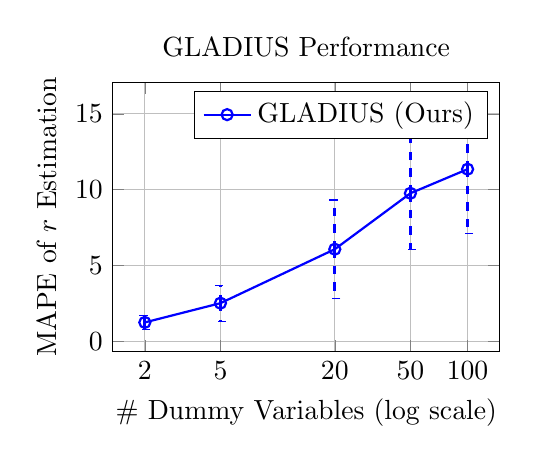
\begin{tikzpicture}
        \begin{semilogxaxis}[
            width=6.5cm, % Adjust width for double column
            height=5cm,
            xlabel={\# Dummy Variables (log scale)},
            ylabel={MAPE of $r$ Estimation},
            title={GLADIUS Performance},
            grid=both,
            xtick={2, 5, 20, 50, 100},
            xticklabels={2, 5, 20, 50, 100},
            ytick={0, 5, 10, 15},
            yticklabels={0, 5, 10, 15},
            mark options={solid},
            legend pos=north east,
            error bars/y explicit,
            error bars/error bar style={line width=1pt, dashed}
        ]

        % AGAD (Ours) with updated values
        \addplot+[mark=o, blue, thick, error bars/.cd, y dir=both, y explicit] coordinates {
            (2, 1.24) +- (0, 0.45)
            (5, 2.51) +- (0, 1.19)
            (20, 6.07) +- (0, 3.25)
            (50, 9.76) +- (0, 3.68)
            (100, 11.35) +- (0, 4.24)
        };
        \addlegendentry{GLADIUS (Ours)}

        \end{semilogxaxis}
        \end{tikzpicture}
    \end{minipage}
    \caption{MAPE of $r$ estimation. The left panel shows the MAPE values in a tabular format, and the right panel visualizes the GLADIUS's performance on a log-scaled x-axis. 1000 trajectories were used for all experiments. Smaller is better; the best value in each row is highlighted.}
    \label{fig:dummy_r_estimation}
\end{figure}
We find that our approach outperforms benchmark algorithms, including SAmQ, IQ-learn, and BC (see Figure \ref{fig:dummy_r_estimation}). Further, as shown in the right panel of Figure \ref{fig:dummy_r_estimation}, the MAPE error exhibits sub-linear scaling with respect to the state dimension size (note that the $x$-axis is in log scale). This suggests that the algorithm can scale well to applications with large dimensional state space.







